
%% bare_conf.tex
%% V1.3
%% 2007/01/11
%% by Michael Shell
%% See:
%% http://www.michaelshell.org/
%% for current contact information.
%%
%% This is a skeleton file demonstrating the use of IEEEtran.cls
%% (requires IEEEtran.cls version 1.7 or later) with an IEEE conference paper.
%%
%% Support sites:
%% http://www.michaelshell.org/tex/ieeetran/
%% http://www.ctan.org/tex-archive/macros/latex/contrib/IEEEtran/
%% and
%% http://www.ieee.org/

%%*************************************************************************
%% Legal Notice:
%% This code is offered as-is without any warranty either expressed or
%% implied; without even the implied warranty of MERCHANTABILITY or
%% FITNESS FOR A PARTICULAR PURPOSE! 
%% User assumes all risk.
%% In no event shall IEEE or any contributor to this code be liable for
%% any damages or losses, including, but not limited to, incidental,
%% consequential, or any other damages, resulting from the use or misuse
%% of any information contained here.
%%
%% All comments are the opinions of their respective authors and are not
%% necessarily endorsed by the IEEE.
%%
%% This work is distributed under the LaTeX Project Public License (LPPL)
%% ( http://www.latex-project.org/ ) version 1.3, and may be freely used,
%% distributed and modified. A copy of the LPPL, version 1.3, is included
%% in the base LaTeX documentation of all distributions of LaTeX released
%% 2003/12/01 or later.
%% Retain all contribution notices and credits.
%% ** Modified files should be clearly indicated as such, including  **
%% ** renaming them and changing author support contact information. **
%%
%% File list of work: IEEEtran.cls, IEEEtran_HOWTO.pdf, bare_adv.tex,
%%                    bare_conf.tex, bare_jrnl.tex, bare_jrnl_compsoc.tex
%%*************************************************************************
\documentclass[conference]{IEEEtran}
\usepackage{graphicx}

\usepackage{filecontents}
\usepackage{tikz}
\usepackage{pgfplots,pgfplotstable} 

\pgfplotsset{
    discard if/.style 2 args={
        x filter/.code={
            \ifdim\thisrow{#1} pt=#2pt
                \def\pgfmathresult{inf}
            \fi
        }
    },
    discard if not/.style 2 args={
        x filter/.code={
            \ifdim\thisrow{#1} pt=#2pt
            \else
                \def\pgfmathresult{inf}
            \fi
        }
    }
}

\begin{filecontents}{comp.dat}
Coord Title Ratio Idx
1 {\rotatebox{70}{MPC555 [14]}}		    0.7	  1 
2 {\rotatebox{70}{ARM7 ETM [14]}}		      0.7   1
3 {\rotatebox{70}{Nexus 5001 [8]}}     	  0.12	1 % cite hopkins
4 {\rotatebox{70}{ }}		          0.66	2
5 {\rotatebox{70}{RATCHET [18]}}		    1.39	3
6 {\rotatebox{70}{VPC3 [3]}}		      1.9	  3
7 {\rotatebox{70}{zcompr [12]}}		    2.1 	3

\end{filecontents}

\begin{document}
%
\title{Value-Prediction-Based Data Trace \\ Compression in BERI} 


\author{\IEEEauthorblockN{Allison Pearce}
\IEEEauthorblockA{St. Edmund's College\\
ap819@cam.ac.uk}}

\maketitle

\begin{abstract}
Extended program traces are a vital tool for the development and analysis of research processors, but they are often
restrictively large. In the case of BERI, a software debugging unit streams trace entries that are transmitted from the processor over
a JTAG serial interface. The low throughput of JTAG makes trace compression particularly valuable. 
This paper describes a hardware implementation of data trace compression for BERI based on the VPC algorithms for 
value-prediction-based trace compression in software. Some elements of VPC proved difficult to translate into hardware or were not adaptable to a streaming application, but the model of using predictors to compress trace data at the hardware level is promising. 
This implementation achieves a 4.6 compression ratio, which is lower than the best academic research implementations, but is
on par with industry standards.

\end{abstract}

\section{Introduction}
% briefly describe BERI
% describe VPC3 in reasonable detail
% especially describe the predictors you ended up using
Traces are a common and often necessary tool for debugging and analyzing processors and software. Address traces track the PC during the execution of a program. Extended traces or data traces provide additional information, such as register content and branch tags. For example, Cambridge's Bluespec Extensible RISC Implementation (BERI) \cite{beri} generates a 256-bit trace entry for each instruction. Needless to say, full data traces can be extremely large, and storing them is a problem. In many systems, including BERI, traces are sent from the processor over a JTAG interface. JTAG's low throughput makes transmission of large amounts of trace data difficult. 

Compression helps to alleviate the storage and transmission problems. Compression can be implemented in hardware or software. Software solutions usually fall into one of two categories: regeneration and compression. Execution-driven solutions like ATOM \cite{ATOM} create binaries that regenerate a new trace on demand, eliminating the need to store the trace at all. However, trace regeneration can be too slow or too expensive for some uses. It is also ISA specific, difficult to port, and can produce unrepeatable results for nondeterministic programs. Compression solves the issues of nondeterminism, but storing compressed traces still requires some disk space. Compressed traces must also be decompressed before they can be used.

Prediction-based compression strategies have been extensively researched. The value-prediction-based compression (VPC) algorithms attempt to minimize the drawbacks of compression and were expressly designed for use with extended traces \cite{vpc}. Value predictors recognize patterns and extrapolate them to predict the values most likely to occur next. Value predictors have been shown to successfully predict the content of CPU registers using fast, simple algorithms \cite{burtscher1999} \cite{gabbay1996} \cite{goeman2001} \cite{rychlik1998} \cite{tullsen1999}. CPU registers tend to contain data similar to that found in data traces. When compressing traces with VPC, value predictors forecast the most likely values for the next PC and extended trace data. If one of the predictors is successful, only the identifier of that value predictor need be written, instead of the full trace entry. Zcompr uses a combination of prediction and interpretation to produce even better compression than VPC \cite{kanev2011}.

VPC and Zcompr, like other software compression strategies, focus on alleviating the problem of \emph{storing} traces. This does not help with the real-time transmission of the trace, and it requires an extra step after the trace has been produced. Hardware compression allows for quick transmission in addition to the reduced storage overhead, and compressing the trace as it is generated means that no additional steps are required after running the processor.

The majority of hardware trace compression techniques focus on address traces. One popular address compression technique is to simply discard contiguous addresses and only report jumps or branches \cite{armspec} \cite{tc1775} \cite{nios2003}. The Nexus 5001 Forum defined a standard for packet-based tracing using a similar address filtering strategy \cite{nexus5001}. These strategies have low overhead and are easy to implement. However, they are limited by the size of the average basic block, which is usually only four or five instructions \cite{rotenberg1999}. Another strategy is to output the difference between each successive address, as in the MIPS PDTrace module \cite{mipspd}. With this method, compression is limited because consecutive instructions cannot be skipped. All of these techniques achieve compression ratios between 5 and 10x \cite{macnamee2000}. Research implementations have achieved significantly better compression results. Kao et al. proposed an LZ-compression-based mechanism that achieves up to 454:1 compression ratios, but at a high complexity (50,000 gates) \cite{kao2007}. Uzelac et al. developed a technique using prediction structures that they claim delivers a 1098:1 compression ratio \cite{uzelac2014}. 

There has been comparatively little research on hardware compression for extended trace data. One system, RATCHET \cite{thatssoratchet}, achieves 20-30:1 compression using a filter cache. However, RATCHET's traces do not capture branching behavior, so they are only reliable for cache behavior analysis, not program analysis. Industry standard compression ratios for for hardware extended trace compression are also on the order of 5-10:1 \cite{hopkins2006}.  

I implemented an extended trace compression mechanism in hardware for BERI based on VPC. The primary goal of compression was to reduce transmission time of traces being streamed by a software debugging application in real time. Because of the inherent differences between hardware and software and in streaming versus storage, VPC could not be perfectly mapped to BERI, but many of the techniques and ideas could. This project demonstrates the feasibility of porting VPC-like prediction algorithms to hardware to achieve compression rates on par with industry standards. 


\section{Background}  
This project's hardware trace compression mechanism was based on the VPC algorithms. VPC is single-pass, which is convenient for storage because it means that the trace need never be fully uncompressed, and it is necessary for compressing traces for transmission during real time streaming. In VPC1, 37 value predictors are applied to the trace data. In the event of a successful prediction, the predictor identification code is written to a file after being further compressed to one byte by a dynamic Huffman encoder. If there are no successful predictions, a flag is written to the file, followed by the unpredictable data. The output of VPC1 is quite compressible, so VPC2 adds a stage to do so. VPC3 uses fewer value predictors and attempts to separately predict both the PC and the trace data. In VPC3, the compressed trace output is divided into four streams that can be further compressed easily: identifiers of PC predictors, unpredictable PC data, identifiers of trace data predictors, and unpredictable trace data. Each of the four streams is then compressed with BZIP2. VPC4 is autogenerated from VPC3 and is faster and better compressing.

In this project, I used some of the same value predictors as VPC3, including the finite context method (FCMn) \cite{sazeides1997}. FCMn hashes the $n$ most recently encountered values to serve as an index into a history table. The value at this index is used as the prediction, hoping that the value that follows in this case will be the same as the value that followed last time this series of $n$ values was encountered. The value at the index is updated with the current value (PC or trace data) if the prediction was wrong. FCMn predictors are useful for long, arbitrary repeating sequences such as PCs. 

Last $n$ value predictors (LnV) \cite{burtscher1999} are another history-based predictor. They simply use the $n$ most recent values as $n$ predictions. LnV predictors perform well with values that alternate or with repeating patterns that have a period of no more than $n$. 

Stride 2-delta predictors (ST2D) \cite{gabbay1996} store the most recent value and the difference (delta) between the most recent value and the one that preceded it. The predicted value is the most recent value plus the difference. It also maintains a second delta value for a second prediction. The second delta is only updated when the same difference is encountered twice in a row. ST2D predictors perform well at predicting numbers in sequences that are incremented or decremented by a fixed amount, such as registers containing loop indices and other types of counters. ST2D predictors were not used in VPC3, but they were found to be advantageous in the BERI compressor. 
\begin{figure}[!b]
\centering
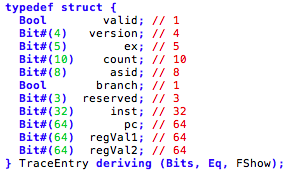
\includegraphics[width=2.5in]{images/trace_types.png}
\caption{BERI's 256-bit TraceEntry struct}
\label{trace_types}
\end{figure}


\section{Compression Implementation}
% something about the fact that it's single-pass
The compression mechanism described here is in some ways a combination of VPC1 and VPC3. Like VPC3, we use a smaller subset of the most successful predictors to forecast both the PC and the trace data. Because the primary use case requires traces to be individually compressed and quickly decompressed for real-time streaming, the strategy of writing to multiple streams and performing BZIP2 compression on the streams is not applicable. Like VPC1, all data is written to the same output. If the predictions are incorrect, a flag and the unpredictable data are transmitted. The predictors used are a subset of those implemented in VPC3. PCs are predicted with FCM1ab (finite context method using the single most recent PC and providing two predictions) and an FCM3ab (finite context method using the three most recent PCs and providing two predictions) for a total of four predictions. Trace data is predicted using L4V (last $n$ value predictor with $n=4$) and stride 2-delta algorithms (six total predictions).  

PC predictions were necessarily implemented with global index information, meaning that the PC predictions are based on the most recent PC values in the whole program's execution. The trace predictions are PC-specific, so the L4V predictor returns the last four trace values encountered at a particular PC, and the ST2D predictor returns the most recent value and delta for the previous occurrence of that PC. If multiple predictions are correct for a particular field, ties are broken by selecting the one with the highest use count.  

Unlike any of the VPC algorithms, I divided the BERI trace data into groups of fields and predicted each group separately. This is because some of the trace fields are much easier to predict than others, and some respond better to different prediction techniques. For example, BERI traces include an increasing \texttt{count} field, which is predicted reasonably well using ST2D but not at all with LnV. If the compressor is designed to treat all trace data as a unit, then correctly predicting all the data but one register, or correctly predicting all of the data but not all with the same predictor, still means that the whole prediction is invalid and the full trace must be transmitted. Predicting groups of fields separately from the rest of the data allows for some compression even when the more difficult predictions fail. The optimal data groups were experimentally determined.

The VPC software algorithms base their predictors on one- or two-level hash tables implemented using C arrays. The hardware implementation relied on BRAM modules to implement hash tables. I did not use any two-level tables in the final hardware compression implementation, because there was no significant benefit to prediction accuracy to offset the additional delay required to index into both levels of the table for lookups and updates. 

The compression module interfaces with BERI's DebugUnit. A secondary goal of the project was to change the existing structure of BERI as little as possible. The compressor provides a GetPut interface where the DebugUnit can enqueue trace entries for compression. A combination of methods and rules performs the lookups and updates with the BRAM predictor tables. The results are packed into a \texttt{CompressedTraceEntry}, a struct containing a valid bit, the four-bit version, three-bit predictor identifiers for the PC and the groups of trace data, and some combination of mispredicted data or padding to fill 256 bits. The DebugUnit expects a 256-bit value, but based on the prediction results encoded in the version field, it will send only the first $n$ bytes in a packet to the software stream tracing application. If all fields are predicted correctly, only three bytes are needed (for the valid bit, version number, and predictor identifiers). If a unit of trace data is mispredicted, the correct value is sent with the message packet. Exceptions occur if the ``easy data"\footnote{The groups of data are further explained in the Results section} is mispredicted or if all of the other data fields are mispredicted; in this case, the original trace entry is sent uncompressed. This is in part to reduce the complication of the decompression logic and in part because some of the sixteen possible versions are reserved, so the number of states that can be communicated to the DebugUnit and decompresser is more limited.  

\section{Evaluation Methods}
\subsection{System}
% TODO get the same info for the lab machine (acs23) that the dude included in his paper
Experiments were performed running a simulation of the BERI processor on an Intel Core i5 running Ubuntu 3.2.0 with four 1197MHz CPUs, 32kB L1 caches, 256kB L2 cache, and 8192kB L3 cache. 
\subsection{Timing Measurements}
As in the analysis of the VPC algorithms, runtime was measured using the UNIX shell \texttt{time} command. The sum of the user and system time is reported, which equates to reporting the CPU time. 
\subsection{Traces} % only if I get some interesting traces
Compression was testing by tracing a BERI simulation running a short program for 268,084 instructions. The program included a variety of operations with implementations of bubble sort, quick sort, and modular exponentiation. It is a weakness of this experiment that only one program was available to run on the simulated BERI processor.

\section{Results}

\begin{figure}
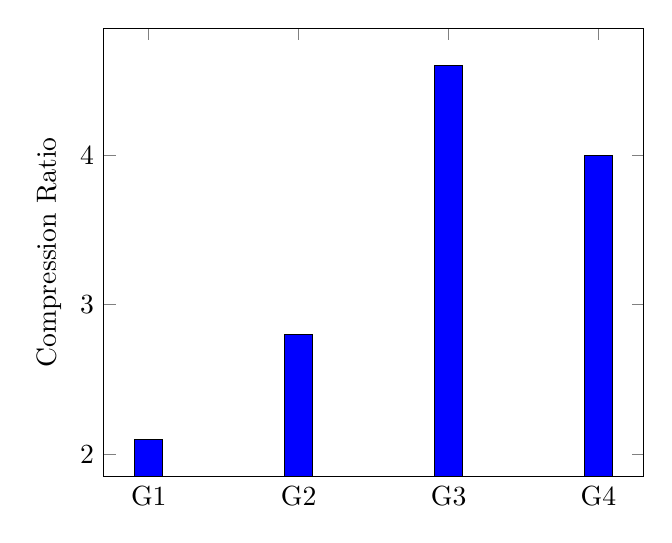
\begin{tikzpicture}
\begin{axis}[
    symbolic x coords={G1, G2, G3, G4},
    xtick=data,
    ylabel=Compression Ratio],
    \addplot[ybar,fill=blue] coordinates {
        (G1,2.1)
        (G2,2.8)
        (G3,4.6)
        (G4,4.0)
    };
\end{axis}
\end{tikzpicture}
\label{group_chart}
\caption{Compression ratios for different prediction groupings of trace fields. All groups predicted ex, asid, branch, reserved, and inst as one group and predicted PC individually. G1 predicted regVal1, regVal2, and count as one unit of data. G2 used regVal1 as a group and regVal2 with count as a second group. G3 predicted count, regVal1, and regVal2 separately. G4 predicted the registers separately and transmitted the count value uncompressed.}
\end{figure}

\subsection{Prediction Groups}
%The fields in a BERI trace are: valid, version, ex, count, asid, branch, reserved, instruction, pc, register value 1, and register value 2. 
The fields in a BERI trace are show in Figure \ref{trace_types}. The count and register fields change in the most complex manner, and we experimented to find the optimal number of predictors and groups of data to maximize compression. Figure 2 shows the compression results for the four best performing groupings. The valid and version fields are necessary for the trace transmission and are not compressed; they contribute 5 bits. In the optimal division, the PC is predicted and compressed individually. The \texttt{ex, asid, branch, reserved} and \texttt{inst} fields almost never change for a given PC and are easy to predict, so they are predicted as one group. Each of the \texttt{count, regVal1,} and \texttt{regVal2} fields are predicted separately. Not shown in the figure are the results attained with the same divisions as the optimal grouping but with the \texttt{count} predictor indexed globally instead of with the PC. That is to say, the ST2D predictor that was used to forecast the \texttt{count} field stored the deltas between the most recent count values, regardless of PC. Using this strategy resulted in extremely poor compression, indicating that \texttt{count} is closely tied to the PC and PC-related data. 

It is also important to note that we had a limited sample of programs to experiment with. These data groups were optimal for the data available, but it is possible that others would perform better when considering a wider variety of program samples. 

\subsection{Compression Rate}
The best performing division of trace data (PC, each register, and count predicted individually, other fields predicted as a unit) produced a compression ratio of 4.6, reducing the volume of data transmitted from the processor by 78\%. Figure 3 compares this compression ratio to some other popular software and hardware compression algorithms. The BERI implementation is on par with the compression mechanisms used in industry, but it is outperformed by research implementations of hardware and especially software data trace compression. 


\subsection{Compression Time}
Running the simulation and test program with no compression took an average of 27.61 milliseconds. With hardware compression, the simulation took 27.71 milliseconds, an increase of only 0.37\%. Modifying the software debugging application to perform the decompression was out of the scope of this project, so unfortunately no data is available on transmission or decompression time. 


\section{Discussion}

% theoretical max/min is fine. mention that we need to get past one byte/entry
% something about software vs hardware or theoretical maxes
% say ratchet sucks because

The BERI compression module could certainly be improved in many ways, but it achieves a compression rate comparable to industry standard. Moreover, RATCHET, the better-performing hardware data trace compressor, has major limitations: namely, its inability to capture branching behavior. Software data tracing has been studied more extensively, but many of the enhancements that made VCP3 and VPC4 so fast and effective are either infeasible or impractical for hardware stream tracing. Still, we can see that the use of value prediction techniques for compression is sound, and prediction is already widely implemented and highly effective in hardware such as branch predictors.  

A major divergence in design from VPC was the decision to predict some fields of the trace data separately instead of as a single unit. This demonstrates a tradeoff between making more accurate predictions and maximizing compression. There are two ways to increase prediction accuracy: use more predictors, or predict more fields individually so as to avoid the complex dynamics of multiple fields changing in different ways. But both of these strategies increase the minimum number of bits needed for predictor identifiers (either in the form of more bits per predictor encoding or more predictor encodings). This increases the minimum size of the transmission when all data is predicted perfectly and thus decreases the maximum compression attainable. 
 
We experimented with finding optimal values for many parameters, but there are almost limitless opportunities to continue tweaking values in hopes of perfecting the predictors. The number of bits in the keys for the BRAMs and the prioritization of the predictors are just two of the values that affect the outcomes of the predictors. Further analysis of these parameters could yield better results. Similarly, the minimum trace size for each entry in this implementation is three bytes. With more experiments and fine-tuning, it would be possible to reduce this number. But any strategy in which each entry is compressed in isolation has a theoretical maximum compression rate equal to the size of the original data to be transmitted (256 in this case, if it were possible to compress each 256-bit trace to one bit of data). VPC3 and VPC4 achieve significantly better results by further compressing the streams with BZIP2, but BZIP2 does not yet have a hardware implementation. Other strategies predict multiple values at once, or use consistent patterns to avoid sending data until the pattern changes. Exploring some form of one of these strategies has the potential to yield far better returns. To have a truly effective compression algorithm competitive with the best research implementations, one needs to be able to send less than one bit of data per trace entry.

 \begin{figure}
 \begin{tikzpicture} 
 \begin{axis}[ 
     ybar,
     xtick={1,...,7},
     xticklabels from table = {comp.dat}{Title},
     xtick align=inside,
     every axis x label/.style={at={(ticklabel cs:0.5)},anchor=north east},
     ylabel=Log(Compression Ratio),
     every axis y label/.style={at={(ticklabel cs:0.5)},rotate=90,anchor=near ticklabel}
 ] 

 %Paper's due today, and I spend unreasonable amounts of time on one graph
 \addplot[ybar, bar shift=0pt, fill=blue,
     discard if not={Idx}{3},
         ] table [ 
     x=Coord,
     y=Ratio
 ] {comp.dat} ;

 \addplot[ybar, bar shift=0pt, fill=red,
     discard if not={Idx}{2},
        ] table [ 
     x=Coord,  
     y=Ratio
 ] {comp.dat} ;

 \addplot[ybar, bar shift=0pt, fill=green,
     discard if not={Idx}{1},
         ] table [ 
     x=Coord, 
     y=Ratio
 ] {comp.dat} ;

 \end{axis} 
 \end{tikzpicture} 
 \label{comparison}
 \caption{Comparison of log of compression rate for a sample of industry and academic implementations. The blue bars indicate industry standard, green bars indicate academic research, and the red bar is for the compressor in this paper. Note that zcompr and VPC3 are software compressors; all others are hardware}

 \end{figure}
  

\section{Future Work}
% decompression lol
% implementing two-level tables? or nah - might not even predict better
The relatively short time frame for this project left many things unimplemented or unexplored. There are two obvious and necessary next steps: alter the software stream tracing application to decompress the traces, and performing synthesis and hardware cost analysis of the compressor module. Other avenues for investigation include finding a hardware analogue to BZIP2 in VPC3 that could be used to further compress the outputs of the predictors and experimenting with other value predictors. It may also be possible to encode multiple trace entries at once by predicting the data for a sequence of instructions. This would require more substantial changes to the hardware DebugUnit and the debugging software, but it would allow for much greater compression. Finally, this compression implementation is specific to the current BERI TraceEntry. Changes to the TraceEntry content could significantly alter the performance of the predictor. It would be ideal to have a more flexible compressor that could handle a variety of trace entry types with different data exhibiting different patterns.

\section{Conclusion}
I implemented a value-predictor-based trace compression mechanism in hardware that delivers a 4.6:1 compression ratio. This ratio is on par with many industry hardware compression implementations. Recent academic approaches achieve compression ratios that are better, but the best of the academic examples are based on similar techniques of prediction. This project was extremely valuable for learning about compression and prediction techniques, learning Bluespec, and understanding more of the fundamental design differences between software programming languages and hardware development languages. 





\bibliographystyle{plain}
\bibliography{acd}


% that's all folks
\end{document}


%\begin{figure}[!t]
%\centering
%\includegraphics[width=2.5in]{myfigure}
% where an .eps filename suffix will be assumed under latex, 
% and a .pdf suffix will be assumed for pdflatex; or what has been declared
% via \DeclareGraphicsExtensions.
%\caption{Simulation Results}
%\label{fig_sim}
%\end{figure}

% Note that IEEE typically puts floats only at the top, even when this
% results in a large percentage of a column being occupied by floats.


% An example of a double column floating figure using two subfigures.
% (The subfig.sty package must be loaded for this to work.)
% The subfigure \label commands are set within each subfloat command, the
% \label for the overall figure must come after \caption.
% \hfil must be used as a separator to get equal spacing.
% The subfigure.sty package works much the same way, except \subfigure is
% used instead of \subfloat.
%


% Note that often IEEE papers with subfigures do not employ subfigure
% captions (using the optional argument to \subfloat), but instead will
% reference/describe all of them (a), (b), etc., within the main caption.


% An example of a floating table. Note that, for IEEE style tables, the 
% \caption command should come BEFORE the table. Table text will default to
% \footnotesize as IEEE normally uses this smaller font for tables.
% The \label must come after \caption as always.
%
%\begin{table}[!t]
%% increase table row spacing, adjust to taste
%\renewcommand{\arraystretch}{1.3}
% if using array.sty, it might be a good idea to tweak the value of
% \extrarowheight as needed to properly center the text within the cells
%\caption{An Example of a Table}
%\label{table_example}
%\centering
%% Some packages, such as MDW tools, offer better commands for making tables
%% than the plain LaTeX2e tabular which is used here.
%\begin{tabular}{|c||c|}
%\hline
%One & Two\\
%\hline
%Three & Four\\
%\hline
%\end{tabular}
%\end{table}


% Note that IEEE does not put floats in the very first column - or typically
% anywhere on the first page for that matter. Also, in-text middle ("here")
% positioning is not used. Most IEEE journals/conferences use top floats
% exclusively. Note that, LaTeX2e, unlike IEEE journals/conferences, places
% footnotes above bottom floats. This can be corrected via the \fnbelowfloat
% command of the stfloats package.



% trigger a \newpage just before the given reference
% number - used to balance the columns on the last page
% adjust value as needed - may need to be readjusted if
% the document is modified later
%\IEEEtriggeratref{8}
% The "triggered" command can be changed if desired:
%\IEEEtriggercmd{\enlargethispage{-5in}}



